\section{Background}
\label{sec:background}
% This chapter begins by providing an overall understanding of Cloud computing and its related research field.
% Then, it narrows down to the Energy-aware resource management problem in Section \ref{C:}.
\subsection{Cloud computing}
Cloud computing is a computing model offers a network of servers to their clients in a on-demand fashion. From NIST's definition \cite{Mell:2011jj}, \textit{"cloud computing is a model for enabling ubiquitous, convenient, on-demand network access to a shared pool of configurable computing resources (e.g., networks, servers, storage, applications and services) that can be rapidly provisioned and released with minimal management effort or service provider interaction."}

To illustrate how it works, considering the case: a Cloud provider builds a data center which contains thousands of servers connected with network. These servers are virtualized which means they are partitioned into smaller units of resources called \emph{Virtual Machines (VMs)} or \emph{Containers} \cite{Felter:2015ki}. A web-based application provider can access and deploy their applications (e.g Endnote, Google Drive and etc.) in these resource units from anywhere in the world. Once the applications start serving, application users can use them without installing on their local computers.


Cloud computing involves three stakeholders (see Figure \ref{fig:stakeholders}): Cloud providers, Cloud users (applications providers), and End (application) users \cite{Jennings:2015ht}. Cloud providers build data centers, provide maintenance and resource management on hardware infrastructures such as servers. Cloud users develop and deploy applications on Cloud infrastructures. End users consumes applications developed by Cloud users and hosted by Cloud providers. 

% Cloud computing has made one critical change in software industry, it separates the role of traditional service provider into service provider and infrastructure provider. As Wei \cite{Wei:2010fn} states, ``one provides the computing of services, and the other provides the services of computing''. Therefore, this separation add one more layer between service provider and users, as: Cloud providers, Cloud users (service providers), and End users \cite{Jennings:2015ht} . 


The detailed goal and objectives of stakeholders are described below. 
\begin{figure}
	\centering
	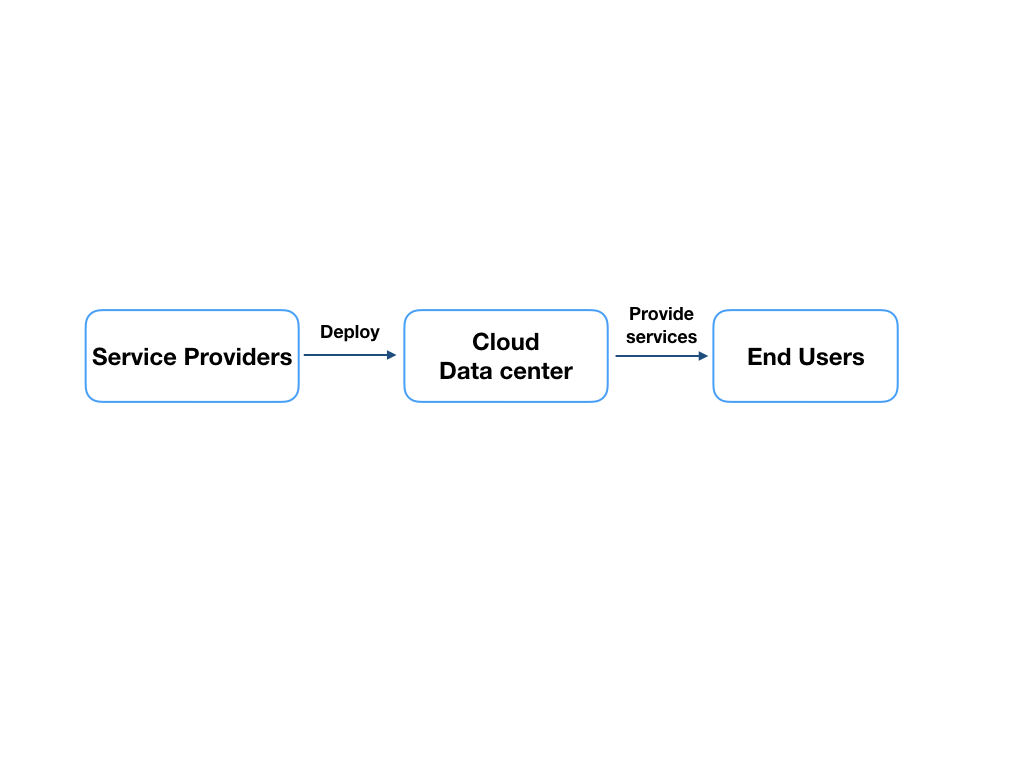
\includegraphics[width=0.7\textwidth]{pics/stakeholders.png}
	\caption{Stakeholders of Cloud computing}
	\label{fig:stakeholders}
\end{figure}

\begin{itemize}
	\item \emph{Cloud providers}' goal is to increase the profit by boosting the income and reducing the expense. Their income comes from Cloud users' rental of servers or \emph{Physical Machines (PMs)} in terms of resource quality (e.g  3.5GHz dual-core CPU), quantity (e.g 3 PMs), and time (e.g 1 year). Therefore, Cloud providers objective is to maximize utilization of computing resources. A high utilization brings two benefits, firstly, it increases income by accommodating more applications in limited resources. Secondly, it cuts the expense of energy consumption by packing applications in a minimum number of PMs so that idle PMs can be turned off. 	
	\item \emph{Cloud users}' goal is also to increase the profit mainly through two objectives, attracting more End users and reduce the expense of resources. The first objective can be achieved by improving the quality of service as well as lower the fee for End users. Either way depends not only on the software entities but also the quality of service (QoS) offered by Cloud provider. The second objective can be achieved by a good estimation of the reserved resources, so that they do not rent insufficient  or too much resources which cause performance degradation or wastage.
	\item \emph{End Users}' goal is to obtain a satisfactory service. It is achieved by signing a Service Level Agreement (SLA) with Cloud users which constrains the performance of the services.
\end{itemize}

Cloud computing has three traditional service models \cite{Mell:2011jj}: Infrastructure as a Service (IaaS), Platform as a Service (PaaS) and Software as a Service (SaaS). The relationship among three service models is showed in Figure \ref{fig:architecture}. 
Service models of Cloud computing are critical in solving energy consumption problem because their distinct ways of managing resources have sever effect on the problem. These distinct ways of resource management mainly result from the responsibilities among stakeholders. 

\begin{figure}
	\centering
	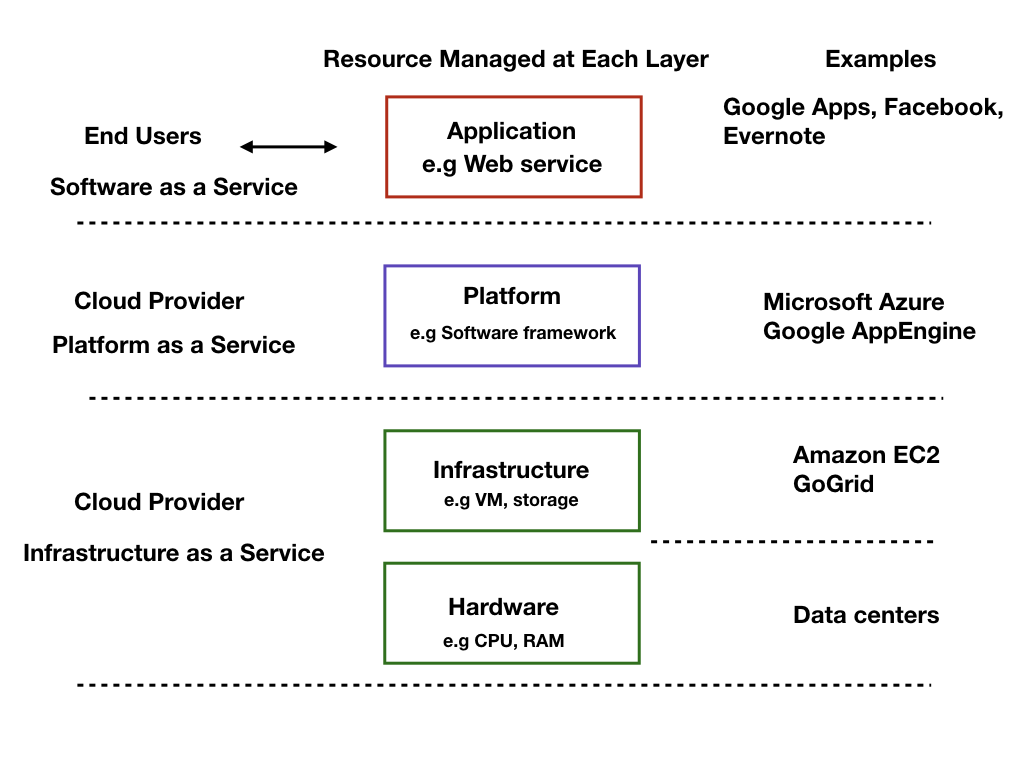
\includegraphics[width=0.9\textwidth]{pics/architecture.png}
	\caption{Cloud computing architecture \cite{Zhang:2010vo}. 
	IaaS provides the fundamental resources such as CPU cores, RAM. The resources are usually wrapped with various types of virtual machine. PaaS provides a software platform sitting on top of IaaS for Cloud users to develop applications. SaaS describes the relationship between applications and End Users.}
	\label{fig:architecture}
\end{figure} 

\begin{itemize}
	\item IaaS, a Cloud provider hosts hardwares such as PMs and cooling infrastructure on behalf of Cloud users. Computational resources are often encapsulated in virtualized computing units called virtual machines (VMs). Cloud providers establish a number of types of VM for simplifying the management. The `type' means a VM contains a certain quantity of resources such as 2-cores and 1 GB RAM.  \emph{Traditional} IaaS and PaaS use VM as the fundamental unit of resources.

	A typical procedure of an application deployment includes several steps.
	Initially, the Cloud user estimates the resources that their applications might consume and selects a type of VM which can satisfy the requirement. After the Cloud user has made the decision, he/she sends requests to Cloud providers for a number of VMs. Finally, Cloud providers received the request, provisioned and allocated these VMs to PMs. 

	% From the resource management perspective, the constraint in allocation of VMs is that the aggregated VMs' resources in a PM cannot exceed the capacity of the PM. After these VMs have been allocated, their types cannot be changed. During the life cycle of an application, Cloud providers can dynamically adjust the locations of VMs, provision new VMs (same type) for the replicas of an application, as well as turning on/off PMs.

	% After receiving the requests, Cloud providers choose a set of PMs which contains sufficient resources, provision the required VMs in them. Then, the VMs are assigned to the Cloud users. Cloud providers manage the VMs by monitoring the resource utilization of VMs and PMs. If a VM has run out of resources, an auto-scaling strategy is used to provision new VMs to Cloud users. Finally, Cloud providers optimize the locations of VMs so that the energy consumption of data center is minimized.


 	\item PaaS, a Cloud provider offers a platform which allows Cloud users to develop, test and deploy their applications on it.

 	From resource management perspective, PaaS is sitting above the IaaS which means the underlying resource is still based on IaaS VM types. Different from IaaS, PaaS takes the responsibility of selecting VMs and allows Cloud users to focus on software development. 

 	% A typical procedure of a Cloud user deploying their applications in an PaaS cloud includes several steps.
 	% In the first step, Cloud users need to provide the initial estimation of the quantity of resources instead of types of VM. Then, Cloud providers determine the types of VM for applications according to the estimated resources.  After this step, resource management system conducts the provisioning and allocating as the same steps in IaaS. During the life cycle of applications, similar to IaaS, Cloud providers can also adjust the location of VMs, add new VMs, and control the status of PMs. Different from IaaS, Cloud providers can change the type of VM for an application as long as the application's performance can be guaranteed.

 	% The system monitors the utilization of a number of PM and VM and through adjustment of their location to optimize the energy consumption of the data center. The input is a list of VMs (e.g CPU cores and RAMs) and a list of PMs. The task is to put the VMs into these PMs so that the VMs only use a minimum number of PMs. The sizes of VMs and PMs are fixed. A system can only adjust which VM is allocated to which PM. A general constraint is the sum of resources of the VMs inside a PM cannot exceed the capacity of the PM.

 	\item SaaS, Cloud users develop applications and deploy them on Cloud so that End users can access them via the Internet. Although this service model does not directly related to the resource management, it provides the fundamental reasons for resource management and optimization: applications receive fluctuated requests from End users. Because of the dynamic nature of workloads, the underlying resources must also be dynamic adjusted to meet the requirement.
\end{itemize}

Overall, Cloud computing has five chacteristics:
\begin{enumerate}
 \item On-demand self-service: A Cloud user can require computing resources (e.g CPU time, storage, software use) without the interaction with Cloud provider.
 \item Broad network access: Computing resources are connected and delivered over the network.
 \item Resource pool: a Cloud provider has a ``pool'' of resources which are normally virtualized servers. In IaaS, it provides predefined sizes of VMs. In PaaS, the resources are `invisible' to Cloud users who have no knowledge or ability to control. 
 \item Rapid elasticity: From the perspective of Cloud users, computing resources are assigned and released in real time. In addition, the resources assign to their software is ``infinite''. Therefore, Cloud users do not need to worried about the scalability of their applications.
 \item Measured Service: Cloud provides an accurate measure of the usage of computing resources. It is fundamental to the pay-as-you-go policy.
\end{enumerate}



\subsection{Virtualization}
\label{sec:virtualization}
Virtualization \cite{Uhlig:2005do} is the fundamental technology that enables Cloud computing. It partitions a physical machine's resources (e.g. CPU, memory and disk) into several independent units called virtual machines (VMs) or containers. This technology rooted back in the 1960s' and was originally invented to enable isolated software testing, because each virtualized unit can provide good isolation which means multiple applications can run in separated VMs within the same PM without interfering each other \cite{Somani:2009ho}. 
Soon, people realized that it can be a way to improve the utilization of hardware resources: With each application deployed in a VM, a PM can run multiple applications. 

% Later, multiple ways of dynamic migration (e.g pre-copy \cite{Clark:2005ud} and post-copy \cite{Hines:2009fv}) of VM were invented, which compresses and transfers a VM from one PM to another. This technique allows resource management in real time which inspires the strategy of server consolidation. 

There are two classes of virtualization (see Figure \ref{fig:comparison}): Hypervisor-based or VM-based and container-based virtualization.

\begin{figure}
	\centering
	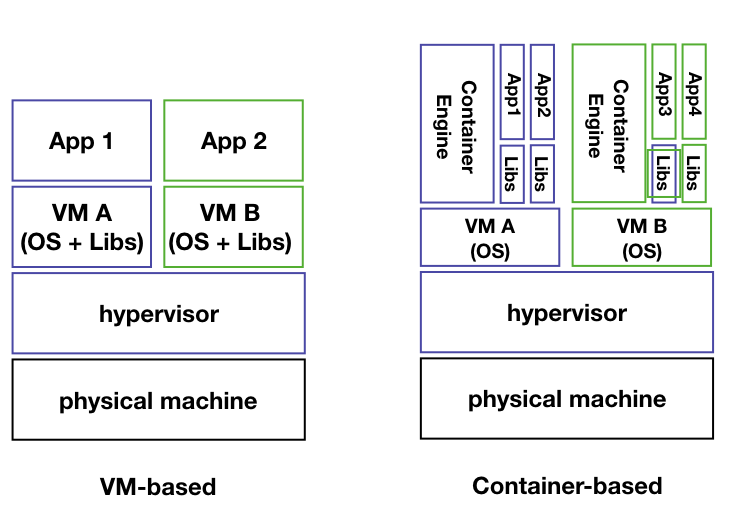
\includegraphics[width=0.7\textwidth]{pics/comparison.png}
	\caption{A comparison between VM-based and Container-based virtualization \cite{Piraghaj:2016bw}}
	\label{fig:comparison}
\end{figure}

\subsubsection{Virtual machine}

A virtualized system includes a new layer of software - the hypervisor or the vrirtual machine monitor (VMM). The VMM arbitrates accesses to the PM's resources so that guests' OS can share them \cite{vm_technology}. In the previous decades VM-based hypervisors such as Xen \cite{Barham:2003cj}, KVM \cite{Kivity:2007wu}, and VMware ESX \cite{Waldspurger:2002db} dominate this field.


\subsubsection{Container}
% It allows applications to have their own separated development environment such as libraries. 

\begin{figure}
	\centering
	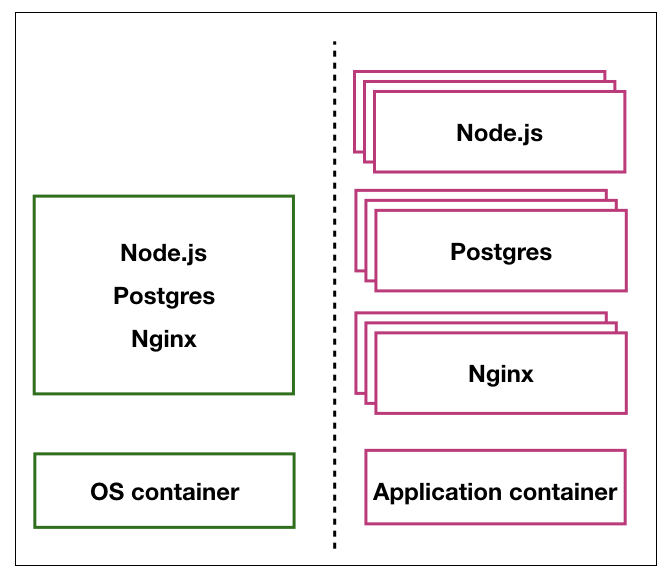
\includegraphics[width=0.4\textwidth]{pics/container_OS_APP.png}
	\caption{A comparison between OS container and Application container \cite{Piraghaj:2017vi}}
	\label{fig:comparison_container}
\end{figure}

Container-based virtualization is also often addressed as 
operating-system-level virtualization. It includes two types of container: OS container and application container \cite{Piraghaj:2017vi}. OS container (as shown in Figure \ref{fig:comparison_container}) can run in both PM and VM. Each container provides an isolated environment. There are mainly three implementations of OS-level of containers: OpenVZ, Google's control groups, and namespace \cite{Rosen:2013wt}.
Google and Facebook have been using OS container for years and being beneficial for its lightweight and fast communication among applications.

In contrast of OS containers, an application container, such as Docker and Rocket, runs a single process. It allows to separate an applications into many components. With application container, it is easy to achieve auto-scaling on a single process. In comparison between OS and application container, the former can be seen as a VM runs multiple applications where each application can has its separated environment (e.g. libraries), while an application container act like a single unit in OS container and it can be allocated in both OS container and VM.

The recent development of application container such as Docker and Kubernetes \cite{Bernstein:2014ur} have attract the attention from both academia and industry. It provides a finer granularity of resource management by enabling an application level of operations including deployment, scaling, and migration.  

% He et al \cite{He:2012im} propose an hierarchical resource management architecture for application container (see Figure \ref{fig:container_architecture}). The major functionality of Cloud controller is to provide a global optimization.

% \begin{figure}
% 	\centering
% 	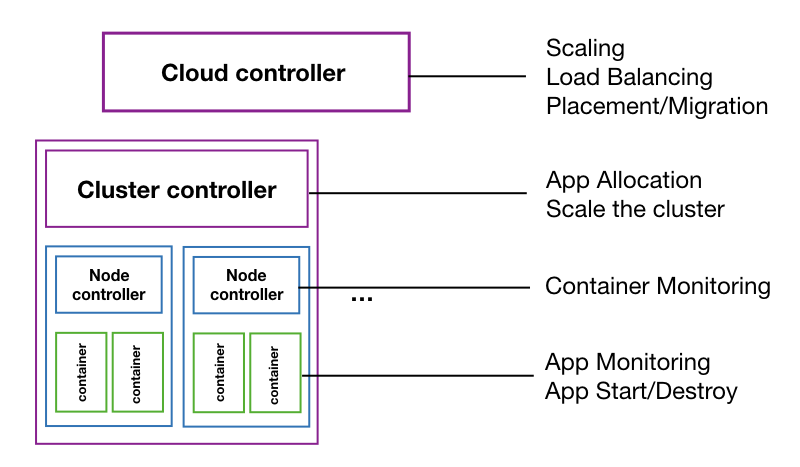
\includegraphics[width=0.7\textwidth]{pics/container-arch.png}
% 	\caption{A resource management architecture of container-based Cloud and the functionalities of each layer.}
% 	\label{fig:container_architecture}
% \end{figure}

\subsubsection{Comparison between Container and VM}
Several research \cite{He:2012im, Felter:2015ki, Xavier:2013fy, Dua:2014bw} have compared VM-based and container-based virtualization. The advantages of container-based virtualization are mainly from three aspects:

\begin{itemize}
	\item Low overhead, containers have a lightweight management. which generate much less overhead than a hypervisor. On the other hand, shared OS system also reduces the overhead on running multiple OSs. 
	\item Containers have a near-native performance of CPU, memory, disk and network. While VM has a poor I/O performance \cite{Shafer:2010vh}: up to 50\% reduction of bandwidth (e.g hard disk and network). This defect also has a negative effect on the migration performance, since a VM-image is ranging from hundreds of MB to several GBs. 
	\item Containers naturally support vertical scaling while VMs do not. Vertical scaling means a container can dynamically adjust its resources under the host's resource constraint.This feature offers a fine granularity management of resources. 
\end{itemize}
	
On the other hand, the disadvantages of containers are categorized in two aspects. Currently, containers have rather poor performance in isolation for memory, disk, and network. Security is immature in containers \cite{Bernstein:2014ur}, therefore, high security required applications are not recommended to be deployed in such systems.

\subsection{Energy Efficiency in Cloud Data centers}

\begin{figure}
	\centering
	\begin{subfigure}[b]{0.45\textwidth}
		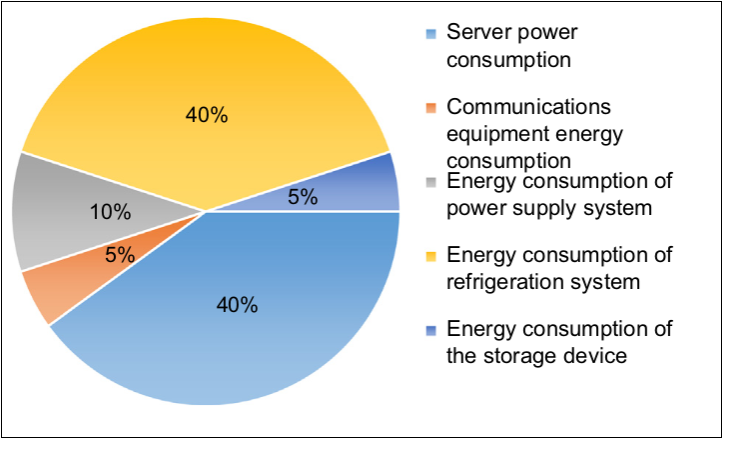
\includegraphics[width=\textwidth]{pics/energyConsumption.png}
		\caption{Energy consumption distribution of data centers \cite{Rong:2016js}}
		\label{fig:consumption}
	\end{subfigure}
	\begin{subfigure}[b]{0.45\textwidth}
		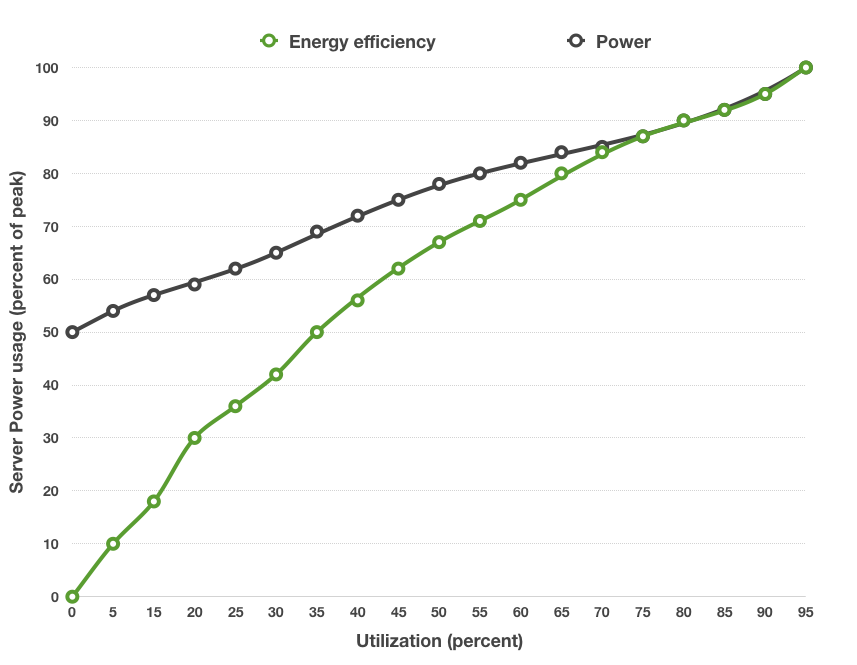
\includegraphics[width=\textwidth]{pics/util.png}
		\caption{Disproportionate between utilization and energy consumption \cite{Barroso:2007jt}}
		\label{fig:unproportional}
	\end{subfigure}
\end{figure} 

Apart from upfront investment, Energy consumption \cite{Kaplan:up01fR-k} is the major expense of data centers. Therefore, it is also the top concern of Cloud providers. Energy consumption is derived from several parts as illustrated in Figure \ref{fig:consumption}. Cooling system and servers or PMs account for a majority of the consumption. A recent survey \cite{Cho:2016kz} shows that the recent development of cooling techniques have reduced its energy consumption and now server consumption has become the dominate energy consumption component. 

According to Hameed et al \cite{Hameed:2016cma}, 
servers are far from energy-efficient. 
The main reason for the wastage is that the energy consumption of servers remains high even when the utilization are low. Therefore, a concept of
\emph{energy proportional computing} \cite{Barroso:2007jt} raised to address the disproportionate between utilization and energy consumption. This leads to 
using virtualization technology to achieve server consolidation.


\subsection{Drawbacks of Traditional Service Models}

There are three characteristics in IaaS which naturally lead to a low resource utilization.
\begin{itemize}
	\item Resource over-provisioning \\
	As previous mentioned, VMs are either selected by Cloud users or automatically selected by software platforms. In either case, it requires an estimation of required resources. However, The accurate estimation is almost impossible because of unpredictable workloads; A simple way is to reserve more resources for ensuring the QoS at peak hours \cite{Chaisiri:2012cv}, rather than completely rely on auto-scaling, simply because auto-scaling is more expensive than reservation. However, the peak hours only account for a short period, therefore, in most of time, resources are wasted. In IaaS, the types of VM are a part of the contract, Cloud providers cannot simply change the type of VMs after provisioning.

	\item Unbalanced usage of resources \\
	Specific applications consume unbalanced resources which leads to vast amount of resource wastage \cite{Tomas:2013iv}. For example, computation intensive tasks consume much more CPU than RAM; a fixed type of VM provides much more RAM than it needs. Because the tasks use too much CPU, they prevent other tasks from co-allocating. This also causes wastage.

	\item Heavy overhead of VM hypervisors and redundant operating systems (OSs) \\
	% Redundant operating systems (OSs) cause vast resource wastage. \\ 
	In VM-based resource allocation, heavy overhead is caused by
	the hypervisor of VMs and the separated operating systems running in the PM. A hypervisor manages and monitors the VMs running on a PM. The overhead of a hypervisor is heavier with the increasing numbers of VM. Redundant operating system is another reason for overhead, as normal applications do not need specific operating systems; Commonly used OSs - such as Linux-based: RedHat, or Windows server versions - are well enough for their needs. Therefore, running applications in separated operating system simultaneously is unnecessary.
\end{itemize}


For traditional PaaS, Cloud providers can adjust the VMs' location and the type of VMs. Therefore, it overcomes the first drawback of IaaS. Because of PaaS is built upon IaaS, the one-on-one relationship between application and VM still exist. PaaS can only select the most suitable type instead of changing their sizes. Therefore, the unbalanced resource problem cannot be solved. In addition, PaaS brings a restriction for the applications deployed on it. PaaS build a software middle-ware to allow Cloud users' development. The middle-ware requires the deployed applications to be compatible with the environment, for example, Google App engine only allows certain programming languages and libraries. Therefore, the generality of PaaS is limited. It is urgent to provide a environment which supports automatic resource management as well as an editable programming environment.


\subsection{Container as a Service}
Container as a Service (CaaS) \cite{Piraghaj:2017vi} is a new service model which is usually considered as a combination of IaaS and PaaS. CaaS uses containers and VM as its fundamental resource allocation unit as shown in Figure \ref{fig:comparison} on the right hand side. 


CaaS has advantages of both IaaS and PaaS  but without their disadvantages. On one hand - similar to PaaS - CaaS allows Cloud providers to manage resource in a fine granularity with containers, therefore, it may lead to high utilization of resources. On the other hand - similar to IaaS - CaaS allows customers to customize their software environment without being constrained by platforms. Therefore, it has more flexibility than PaaS.
	
\subsection{Bilevel Optimization}

\subsection{Vector Bin Packing Problem}
A d-dimensional Vector Bin Packing Problem ($VBP_d$), give a set of items $I^1, I^2, \dots, I^n$ where each item has $d$ dimension of resources represented in real number $I^i \in R^d$. A valid solution is packing $I$ into bins $B^1, B^2, \dots, B^k$. For each bin and each dimension, the sum of resources can not exceed the capacity of bin. The goal of Vector Bin Packing problem is to find a valid solution with minimum number of bins. $VBP_d$ is an NP-hard problem.

\section{Server consolidation}

Server consolidation packs a number of VMs on fewer number of PMs to improve the resource utilization and decrease the energy consumed by PMs. It is often applied to solve the problem of physical server sprawl \cite{Khanna:2006vq}: a situation that more PMs are used in a low-utilized way. 


% \textcolor[Maroon]{Why Server consolidation?}
% Physical server sprawl not only wastes valuable computing resources but leads to a waste of energy, as Hameed et al \cite{Hameed:2016cma} addressed, even at a low level of 10\% of CPU utilization, PMs still consume more than 50\% of its peak time. 
% In addition, Han et al \cite{Han:2017jz} state that average resource utilization of PMs  is usually between 10\% to 50\%
% of its capacity. Server consolidation is often used to solve the disproportionate between utilization and energy consumption \cite{Barroso:2007jt}.

% \textcolor[Maroon]{How to do server consolidation?}
From a broad technologies perspective, there are generally two technologies can be used to achieve server consolidation: clustering and virtualization. Clustering is used in a situation that the applications running in PMs are I/O intensive. This is because current virtualization technologies  such as KVM \cite{Kivity:2007wu} or Xen \cite{Barham:2003cj} have a 20\% to 55\% of reduction of I/O bandwidth (e.g disk reads and writes, network bandwidth) in comparison with non-virtualized PM \cite{Shafer:2010vh}. Virtualization is more suitable for applications which require little CPU utilization (e.g 15\%) and low I/O needs. Web services are mostly categorized into this group. Three major benefits of virtualization make it be the first choice for web-based application consolidation: No reliance on hardware, easy to provision and live migration.

\begin{figure}
	\centering
	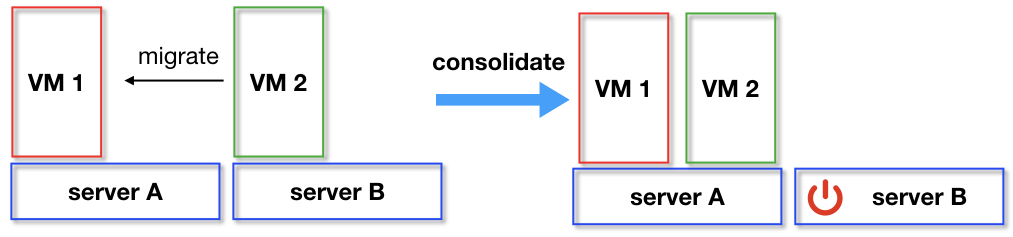
\includegraphics[width=0.7\textwidth]{pics/consolidate.png}
	\caption{A Server Consolidation example: Initially, each PM runs an application wrapped with a VM in a low resource utilization state. After the consolidation, both VMs are running on PM A, so that PM B is turned off to save energy \cite{Barroso:2007jt}.}
	\label{fig:consolidation}
\end{figure}

Virtualization-based Server consolidation \cite{Zhang:2010vo} utilized a dynamic migration technique (e.g pre-copy \cite{Clark:2005ud} and post-copy \cite{Hines:2009fv}) to resolve the low utilization problem by gathering applications into a fewer number of PMs (see Figure \ref{fig:consolidation}), so that the resource utilization of PMs are maintained at a high level. In the meanwhile, idle PMs can be turned off to save energy. Consolidation dramatically improves hardware utilization and lowers PM and cooling energy consumption. 

Server consolidation can be done in two ways: Static and Dynamic \cite{Xiao:2015ik, Verma:2009wi} which are applied in different resource management scenarios (discuss in next section). In some scenarios, for example: new application initialization and global consolidation, involve large number of variables, therefore, it is very time-consuming job and often conducted in an off-line fashion. In other scenarios, when PMs are overloading or underloading, it requires fast a decision-making to migrate one or more VMs to reduce the burden on overloaded PM or improve the utilization. It migrates one VM at a time with a dynamic method. 



\subsection{General Server Consolidation Scenarios}

The server consolidation in data center can be applied to three \cite{Svard:2015ic, Mishra:2012kx} scenarios: Application initialization, Prediction and Global consolidation, and Dynamic resource management (see Figure \ref{fig:management}). 

\begin{figure}
	\centering
	\begin{subfigure}[b]{0.9\textwidth}
		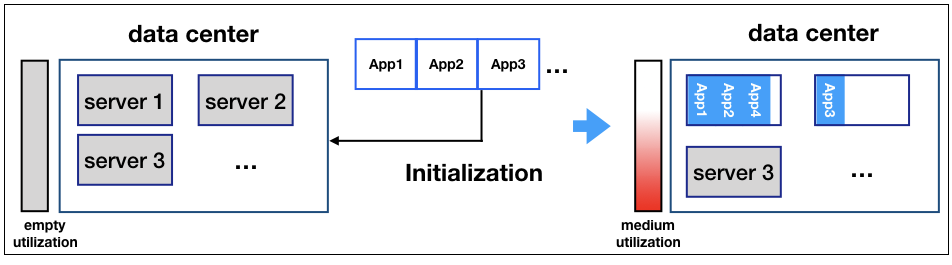
\includegraphics[width=\textwidth]{pics/initialization.png}
		\caption{Initialization}
	\end{subfigure}
	\begin{subfigure}[b]{0.9\textwidth}
		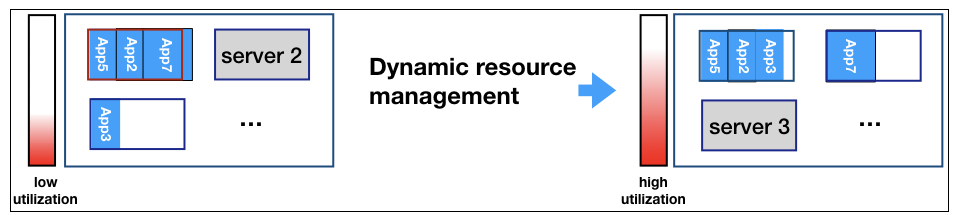
\includegraphics[width=\textwidth]{pics/dynamic_resource.png}
	\caption{Dynamic resource management}
	\end{subfigure}
	\begin{subfigure}[b]{0.9\textwidth}
		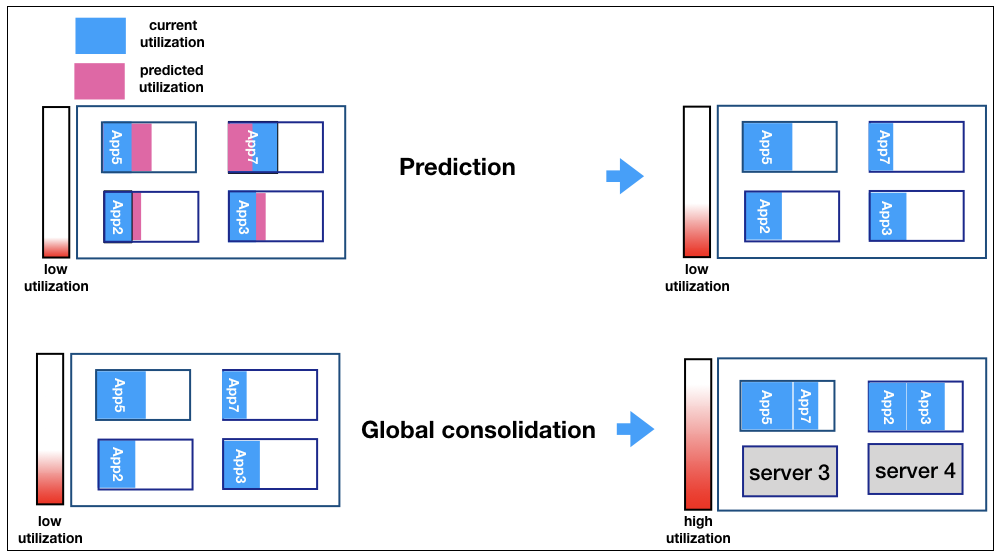
\includegraphics[width=\textwidth]{pics/predict_consolidate.png}
	\caption{Prediction and Consolidation}
	\end{subfigure}
	\caption{Three scenarios of resource management}
	\label{fig:management}
\end{figure}

% Data center constantly receives new requests for applications initialization. Once the new applications have been allocated, the utilization begins to drop. This is because, initially, applications are compactly allocated on PMs. As old applications instance are released because of canceling, the compact structure become loose. Dynamic resource management is a process which can slow the utilization from decreasing. It consolidates by re-allocating one application at a time. Finally, global consolidation is conducted periodically to dramatically improve the resource utilization.
\begin{enumerate}
	\item \emph{Application initialization} is applied when new applications or new VMs arrive and the problem is to allocate them into a minimum number of PMs.

	In this problem, a set of applications or VMs are waiting in a queue. The resource capacity of the PM and usage by applications are characterized by a vector of resource utilizations including CPU, memory and etc. Then, the allocation system must select a minimum number of PMs to accommodate them so that after the allocation, the resource utilizations remain high. The problem is to consider the different combinations of applications so that the overall resource utilization is high. This problem is naturally modeled as a static bin-packing problem \cite{CoffmanJr:1996ui} which is a NP-hard problem meaning it is unlikely to find an optimal solution of a large problem. 

	\item \emph{Prediction and Global consolidation} is conducted periodically to adjust the current allocation of applications so that the overall utilization is improved.

	In this problem, time is discrete and it can be split into basic time frames, for example: ten seconds. A periodical operation is conducted in every $N$ time frames.
	A cloud data center has a highly dynamic environment with continuous arriving and releasing of applications. Releasing applications cause hollow in PMs; new arrivals cannot change the structure of current allocation. Therefore, after the initial allocation, the overall energy efficiency is likely to drop along with time elapsing. 

	In prediction, an optimization system takes  the current applications' utilization records as the input. Make a prediction of their utilization in the next period of time. 
	In Global consolidation, based on the predict utilization and the current allocation - including a list of applications/VMs and a list of PMs, the system adjusts the allocation so that the global resource utilization is improved.

	In comparison with initialization, instead of new arrivals, the global consolidation considers the previous allocation. Another major difference is that global consolidation needs to minimize the differences of allocation before and after the optimization. This is because the adjustment of allocation relies on a technique called live migration \cite{Clark:2005ud}, and it is a very expensive operation because it occupies the resources in both the host and the target. Therefore, global optimization must be considered as a time-dependent activity which makes the optimization even difficult.

In comparison with dynamic consolidation, global consolidation takes a set of VMs as input instead of one. Therefore, it is time consuming and often treated as a static problem.
	\item \emph{Dynamic resource management} 
 	is applied in three scenarios. \textbf{First},  it is applied when a PM is overloading. In order to prevent the QoS from dropping, an application is migrated to another PM. This is called hot-spot mitigation \cite{Mishra:2012kx}. \textbf{Second}, it is applied when a PM is under-loading. Under-loading is when a PM is in a low utilization state normally defined by a threshold. At this moment, all the applications in the under-loading PM are migrated to other active PMs, so the PM becomes empty and can be turned off. This is called dynamic consolidation. \textbf{Third}, it is applied when a PM having very high level of utilization while others having low. An adjustment is to migrate one or more application from high utilized PMs to low ones. This is called load balancing.

	No matter which scenario it is, a dynamic resource management always involves three steps . 
	\begin{itemize}
		\item \emph{When to migrate?} refers to determine the time point that a PM is overloaded or underloaded. It is often decide by a threshold of utilization.
		\item \emph{Which application to migrate?} refers to determine which application need to be migrated so that it optimize the global energy consumption.
		\item \emph{Where to migrate?} refers to determine which host that an application is migrated to. This step is called dynamic placement which is directly related to the consolidation, therefore, it is decisive in improving energy-efficiency. 
	\end{itemize}

	Among three operations, dynamic placement is a dynamic and on-line problem.
	The term ``dynamic'' means the request comes at an arbitrary time point. An on-line problem is a problem which has on-line input and requires on-line output \cite{Borodin:uQcy_H6C}. It is applied when a control system does not have the complete knowledge of future events.

	There are two difficulties in this operation, firstly, dynamic placement requires a fast decision while the search space is very large (e.g hundreds of thousands of PMs). Secondly, migrate one application at a time is hard to reach a global optimized state.

\end{enumerate}

Finally, a consolidation plan includes four major items:
			\begin{enumerate}
				\item A list of existing PMs after consolidation
				\item A list of new virtual machines created after consolidation
				\item A list of old PMs to be turned off after consolidation
				\item The exact placement of applications and services
			\end{enumerate}


% \subsection{VM-based Static Consolidation Techniques}
% \label{sec:static}

% Static initialization, is also frequently referred to initial placement problem \cite{Jennings:2015ht}. Whenever a request for provisioning of applications by one or more Cloud users. The resource management system schedules the applications into a set of PMs. Currently, most state-of-the-art research focus on VM-based placement, in this case, applications are installed in VMs. Therefore, ``application placement'' and ``VM placement'' are used interchangeable in the literature. 

% In energy-aware resource management, the initialization has the objective of minimizing the used PMs. In literature, the static initialization problem is often modeled as the vector bin packing problem. Each application represents an item and PMs represents bins.

\section{Related Work}
\subsection{Initialization (VM Placement)}
In energy-aware resource management, the initialization has the objective of minimizing the used PMs. In literature, the static initialization problem is often modeled as the vector bin packing problem. Each application represents an item and PMs represents bins.


Gao et al \cite{Gao:2013gg} and Ferdaus et al \cite{Ferdaus:2014ep} both propose an Ant Colony Optimization based metaheuristic. They considered three resources CPU, memory, and network I/O with two objectives: minimizing power consumption and resource wastage. They model multi-dimensional resource utilization based on vector algebra complementary resource utilization capturing technique \cite{Mishra:2011bz}. They propose a \emph{Resource Imbalance Vector} to capture the imbalance among three resources. Meanwhile, they apply a linear energy consumption function to capture the relationship between CPU utilization and energy \cite{Fan:2007jr}. Their solution was compared with four algorithms: Max-Min Ant System, a greedy-based approach, and two First Fit Decreasing-based methods. The results show that their proposed algorithm has much less wastage than other algorithms.

Xu and Fortes propose a multi-objective VM placement approach with three objectives: minimizing total resource wastage, power consumption and thermal dissipation costs. They applied an improved grouping genetic algorithm with fuzzy multi-objective evaluation. Their wastage by calculating as differences between the smallest normalized residual resource and the others. They also applied a linear power model to estimate the power consumption \cite{Lien:2007it}.  They conduct experiments on synthetic data and compare with six traditional approaches including First Fit Decreasing (FFD), Best Fit Decreasing (BFD) and single-objective grouping GA. The results showed the superior performance than other approaches. 

% Because of its NP-hard nature, several researchers propose well-known bin-packing heuristics
% First Fit (FF), First Fit Decreasing (FFD), Best Fit (BF) and etc. These algorithms have constant-factor approximation to bin-packing problems. However, VM placement is more complex than bin-packing problem \cite{Mann:2015ua}, 

% Panigraph et al \cite{Panigrahy:2011wk} study variants of First Fit Decreasing (FFD) algorithms and inspired by bad isntances for FFD-type algorithms, they propose a geometric heuristics which outperform FFD-based heuristics in most of cases.

% \subsection{VM-based Dynamic Consolidation Techniques}
% \label{sec:dynamic}

% \section{Container-based Consolidation Techniques}
% Initialization is one of the major step in resource management. It can be considered as a static problem \cite{Jennings:2015ht} or dynamic problem \cite{Beloglazov:2012bw}. 
% As we discussed in the previous section, a dynamic allocation normally cannot gives a global optimized solution of a batch of tasks. Therefore, in the context of maximizing the energy efficiency of a data center, we category initialization into a static optimization approach.
\subsection{Periodic consolidation}

Murtazaev and Oh \cite{Murtazaev:2011ue} propose a Sercon algorithm which is a heuristic based on First and Best Fit to solve the periodic consolidation problem. They consider two resources CPU and memory with two optimization objectives, minimizing the energy consumption and the number of migration. They conduct experiments on synthetic data and compare with FFD. The results indicate that Sercon outperforms FFD in migration efficiency, meanwhile, the numbers of nodes used in Sercon and FFD are almost the same.

\subsection{VM-based Dynamic Consolidation Techniques}
\label{sec:dynamic}

\subsection{Container-based Consolidation Techniques}
\subsubsection{Initilization (Container Placement)}
% Initialization is one of the major step in resource management. It can be considered as a static problem \cite{Jennings:2015ht} or dynamic problem \cite{Beloglazov:2012bw}. 
% As we discussed in the previous section, a dynamic allocation normally cannot gives a global optimized solution of a batch of tasks. Therefore, in the context of maximizing the energy efficiency of a data center, we category initialization into a static optimization approach.

% % Previous research mainly use heuristic to solve this problem. 
% Mesos \cite{Hindman:2011ux} is a platform for sharing commodity clusters between cluster computing frameworks such as Hadoop and MPI. It has a two-level of resource allocation architecture where a master node and several slave node. A master node only decides how many resources to offer to each framework (slave) based on fair sharing policy \cite{Ghodsi:2011vm}. Each slave node belongs to a cluster framework and it makes the decision of which resources to use. Each framework has to define its allocation policy. Mesos focus on sharing resources across multiple frameworks and has a better scalability since it deligates the application placement to decentralised slave nodes. The main problem for Mesos is that it does not consider energy consumption for Cloud providers with user-defined allocation policy.

% Piraghaj et al \cite{Piraghaj:2016bw} propose an architecture for container-based resource management. Their allocation approach is policy-based, where it allocates each VM with containers until its estimated utilization above 90\%. This heuristic is similar to First Fit, it is fast but does not guarantee global optimal.

% \subsection{Traditional Approaches}
% \subsection{EC Approaches}

% \section{}
% \textcolor{Maroon}{Why this field is important.}

% Cloud computing has made one critical change in software industry, it separates the role of traditional service provider into service provider and infrastructure provider. As Wei \cite{Wei:2010fn} states, ``one provides the computing of services, and the other provides the services of computing''. Therefore, this separation add one more layer between service provider and users, as: Cloud providers, Cloud users (service providers), and End users \cite{Jennings:2015ht} (see Figure \ref{fig:stakeholders}). 

% This separation of role has completely reformed the software industry \cite{Buyya:2009ix} by providing three major benefits to Cloud users. First, Cloud users do not need upfront investment in hardwares (e.g servers and networking devices) and pay for hardwares' maintenance. Second, Cloud users will not worried about the limited resources will obstruct the performance of their services when unexpected high demand occurs. The elastic nature of cloud can dynamic allocate and release resources for a service. In addition, Cloud users can pay as much as the resource usage under a \emph{pay-as-you-go} policy. Third, Cloud users can publish and update their applications at any location as long as there is an Internet connection. These advantages allow anyone or organization to deploy their softwares on Cloud in a reasonable price. 




% In this thesis, we focus on a core issue of helping Cloud providers to increase their profits. This goal can be done by two ways, attracting more Cloud users to use Cloud services and reducing the expense.








% Service models of Cloud computing are critical in solving energy consumption problem because their distinct ways of managing resources have severe effect on the problem. These distinct ways of resource management mainly result from the responsibilities among stakeholders. 

% There are three traditional service models \cite{Mell:2011jj} which describe the responsibilities among stakeholders: Infrastructure as a Service (IaaS), Platform as a Service (PaaS) and Software as a Service (SaaS). The architecture of Cloud computing is illustrate in Figure \ref{fig:architecture}.

% \begin{itemize}
% 	\item IaaS, a Cloud provider hosts hardwares such as PMs and cooling infrastructure on behalf of Cloud users. A Cloud provider also provides maintenance, management of hardware resources. 

% 	In IaaS, Cloud provider offers the fundamental resources such as CPU cores, RAMs, and network bandwidth. These resources are often encapsulated in virtualized computing units called virtual machines (VMs). Cloud providers establish a number of types of VM for simplifying the management. The `type' means a VM contains a certain quantity of resources such as 2-cores and 1 GB RAM.  \emph{Traditional} IaaS and PaaS use VM as the fundamental unit of resources.

% 	A typical procedure of a Cloud user deploying their applications in an IaaS cloud includes several steps.
% 	Initially, Cloud users estimate the resources that their applications might consume and select a type of VM which can satisfy the requirement. After Cloud users have made the decisions, they send requests to Cloud providers for a number of VMs. Finally, Cloud providers received the request, provisioned and allocated these VMs to PMs. 

% 	From the resource management perspective, the constraint in allocation of VMs is that the aggregated VMs' resources in a PM cannot exceed the capacity of the PM. After these VMs have been allocated, their types cannot be changed. During the life cycle of an application, Cloud providers can dynamically adjust the locations of VMs, provision new VMs (same type) for the replicas of an application, as well as turning on/off PMs.

	% After receiving the requests, Cloud providers choose a set of PMs and allocate the required VMs in them. Then, Cloud users can access the VMs through remote consoles. Cloud providers manage the VMs by monitoring the resource utilization of VMs and PMs. If a VM has run out of resources, an auto-scaling strategy is automatically applied to duplicate the users' VM. Finally, Cloud providers optimize the locations of VMs by consolidating them into a minimum number of PMs.


 	% \item PaaS, a Cloud provider builds a software platform on top of hardwares provided by IaaS. This platform allows a complete life-cycle of software development including development, testing and deployment.

 	% From resource management perspective, PaaS is sitting above the IaaS which means the underlying resource is still based on IaaS VM types. Different from IaaS, PaaS takes the responsibility of selecting VMs and allows Cloud users to focus on software development. 

 	% A typical procedure of a Cloud user deploying their applications in an PaaS cloud includes several steps.
 	% In the first step, Cloud users need to provide the initial estimation of the quantity of resources instead of types of VM. Then, Cloud providers determine the types of VM for applications according to the estimated resources.  After this step, resource management system conducts the provisioning and allocating as the same steps in IaaS. During the life cycle of applications, similar to IaaS, Cloud providers can also adjust the location of VMs, add new VMs, and control the status of PMs. Different from IaaS, Cloud providers can change the type of VM for an application according to it needs.

 	% The system monitors the utilization of a number of PM and VM and through adjustment of their location to optimize the energy consumption of the data center. The input is a list of VMs (e.g CPU cores and RAMs) and a list of PMs. The task is to put the VMs into these PMs so that the VMs only use a minimum number of PMs. The sizes of VMs and PMs are fixed. A system can only adjust which VM is allocated to which PM. A general constraint is the sum of resources of the VMs inside a PM cannot exceed the capacity of the PM.

 	% \item SaaS describes the relationship between Cloud users and End users. End users create workloads for applications. Although this service model does not directly related to the resource management, it provides the fundamental reasons for resource management and optimization. Because of the dynamic nature of workloads, the underlying resources must also be dynamic adjusted to meet the requirement.
% \end{itemize}



% \textcolor{Maroon}{Describe the current ``hot topics'' in the field}

% \subsection{Research Fields in Cloud Computing}
% Cloud computing paradigm has been applied for over ten years, however, many problems have been fully addressed and new challenges has emerged along with new technologies. We summarize some of the hot research fields.

% \subsubsection{Automated service provisioning}
% The key functionality of Cloud computing is to provide an elastic resource management for applications. Cloud users desire a complete automated service provisioning which automatically allocate and release resources for applications that satisfies the service level objective (SLOs). 

% Current automated service provisioning normally involves three steps \cite{Zhang:2010vo}: 
% (1) Constructing a performance model which can predict the need of resources of a given application. (2) Periodically predict the future resource requirement of the application using the model. (3) Automatically allocating resources to the application.

% There are multiple difficulties in this problem. First problem is the mapping between SLOs such as Quality of Service (QoS) requirements: throughput, response time and etc, to low level hardwares such as CPU and memory requirements. This problem is often addressed as Resource Demand Profiling. Approaches are categorized into model-driven, where a predefined model is used to identify the resources' requirement of applications; or statistical techniques which use machine learning algorithms to predict the requirement in the future.

% In the model-driven category, Urgaonkar and et al \cite{Urgaonkar:2005uo} that use a queuing model to determine the resources (each server as the resource unit) for multi-tier application. They model each server as as a G/G/1 queuing system; Bennani and Menasce \cite{Bennani:2005wd} also propose a multiclass queuing network models for both online transactions applications and batch processing applications. 

% In statistical approaches, Li and et al \cite{Li:2011cx} develop a trace-and-replay tool called CloudProphet to predict a legacy application's performance. It monitors the performance of the application locally and replays the workload in the cloud for prediction. Gong and et al. \cite{Gong:2010td} use a signal processing algorithm - Fast Fourier Transform to detect 
% repeating resource usage patterns, and a statistical learning algorithm - discrete-time Markov chain to build short-term demand predictions.

% Furthermore, the decisions are often made in an on-line fashion to trigger the allocation and de-allocation of resources in order to satisfy the fluctuate workload over multiple time scales \cite{Crovella:1997tr}. 



% \subsubsection{Virtual machine migration}
% \subsubsection{Server consolidation}
% \subsubsection{Energy management}
% \subsubsection{Novel cloud architectures}

% \subsection{Container as a Service}
% Our proposed optimization approaches are based on a new service model: 

% Before explaining the details of resource management strategies, we first illustrate several characteristics of resource management in IaaS.
% Firstly, we illustrate the disadvantages of traditional IaaS and PaaS and discuss the reasons of why current approaches cannot completely overcome these problems. From there, we explain why CaaS is a prescription of their problems.




% Specifically, the profit can be improved by reducing the energy consumption. A direct way to reduce energy consumption is to always use a minimum number of Physical machines (PMs) hosting applications. This is because the more PMs are running, the more energy they are 
% consumed.



% Cloud computing is derived from a few computing paradigms including Grid computing, service computing and etc. Grid computing allow their users to run a large-scale computational intensive tasks on a geographically distributed computing resources. Cloud computing is similar to grid computing of utilizing a group distributed
% comtpuing resources. Unlike grid takes each computer as an individual resource, Cloud computing virtualizes the Physical resources into VMs and provides a centralized resource management. Service computing, including Service Oriented Architecture (SOA) and Web services, focus on constructing large scale Web-based application using the Internet. In SOA, web services are the building blocks of softwares and they can be distributed developed, deployed and composited through the Internet. The technologies, such as SOAP and REST, enables Web serivces.










% Service computing such as Service Oriented Architecture and Web Services, focus on the seamless business processes. 

% The purpose of Cloud computing is to reduce the cost of ``in-house'' 




% The separate responsibility between Cloud providers and Cloud users has completely reformed the software industry \cite{Buyya:2009ix} by providing three major benefits to Cloud users.
% First, Cloud users do not need upfront investment in hardwares (e.g PMs and networking devices) and pay for hardwares' maintenance. Therefore, it eliminates the risk of initial investment.
% Second, Cloud users do not need to worry about the limited resources which can obstruct the performance of their services when unexpected high demand occurs. Cloud providers off an elastic nature of Cloud which can dynamic allocates and releases resources for a software.  Cloud users only need to pay the resources that they have used under a \emph{pay-as-you-go} policy. Third, Cloud users can publish and update their applications at any location as long as there is an Internet connection. These advantages allow anyone or organization to deploy their softwares on Cloud in a reasonable price. 

% As previous section mentioned, our goal in this thesis is to help Cloud providers to increase their profit from data centers. Specifically, we focus on how to save money by cutting expenses of Cloud data centers. 
% Cloud providers have two ways of achieving this goals, one is to provide better Quality of Service (QoS) service such as high throughput, low latency, and high availability, to attract more Cloud users to use Cloud services. The other way is to save money 
% Each stakeholder has their objectives.  End users consume application. They require a guarantee quality of softwares including functional requirements which are the functionalities defined by Cloud users, and non-functional requirements such as availability, security, and network latency. Cloud users develop and deploy softwares on Cloud. They provide functional correct softwares and they also desire the non-functional requirements of softwares can be satisfied by Cloud resources. Cloud providers offer low-level resources such as computational power, storage and network bandwidth. Cloud providers want to increase their profit by attracting more Cloud users to use Cloud services and reducing the expense caused
% \begin{figure}[H]
% 	\centering
% 	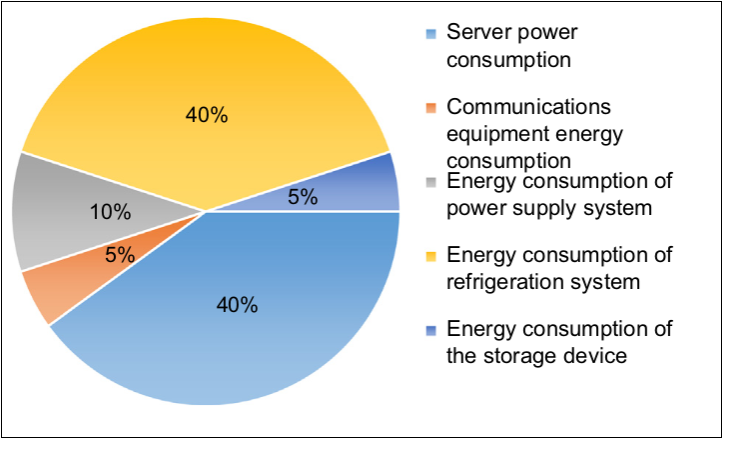
\includegraphics[width=0.5\textwidth]{pics/energyConsumption.png}
% 	\caption{Energy consumption distribution of data centers \cite{Rong:2016js}}
% 	\label{fig:consumption}
% \end{figure} 








% \subsection{Resource Management in IaaS}
% The resource management in IaaS can be roughly separated into three \cite{Svard:2015ic, Mishra:2012kx} which are applied in different scenarios: Application initialization, Prediction and Global consolidation, and Dynamic resource management (see Figure \ref{fig:management}). 

% \begin{figure}
% 	\centering
% 	\begin{subfigure}[b]{0.9\textwidth}
% 		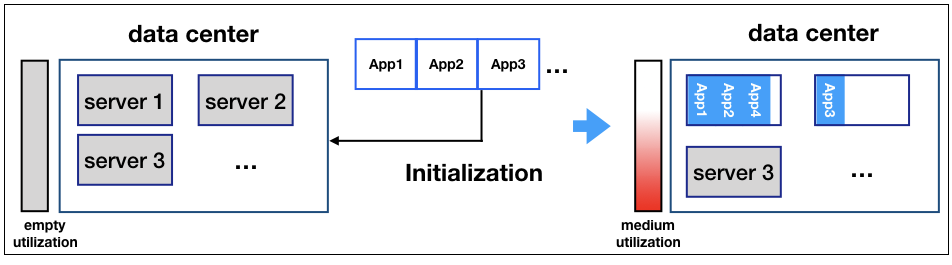
\includegraphics[width=\textwidth]{pics/initialization.png}
% 		\caption{Initialization}
% 	\end{subfigure}
% 	\begin{subfigure}[b]{0.9\textwidth}
% 		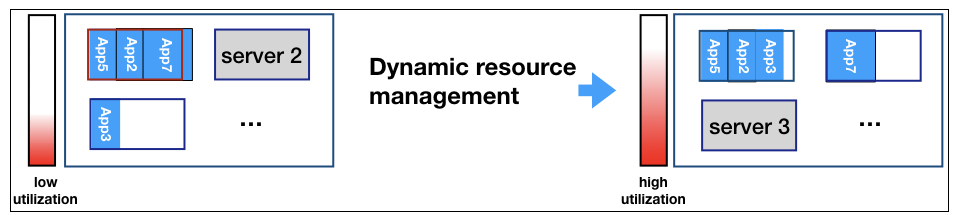
\includegraphics[width=\textwidth]{pics/dynamic_resource.png}
% 	\caption{Dynamic resource management}
% 	\end{subfigure}
% 	\begin{subfigure}[b]{0.9\textwidth}
% 		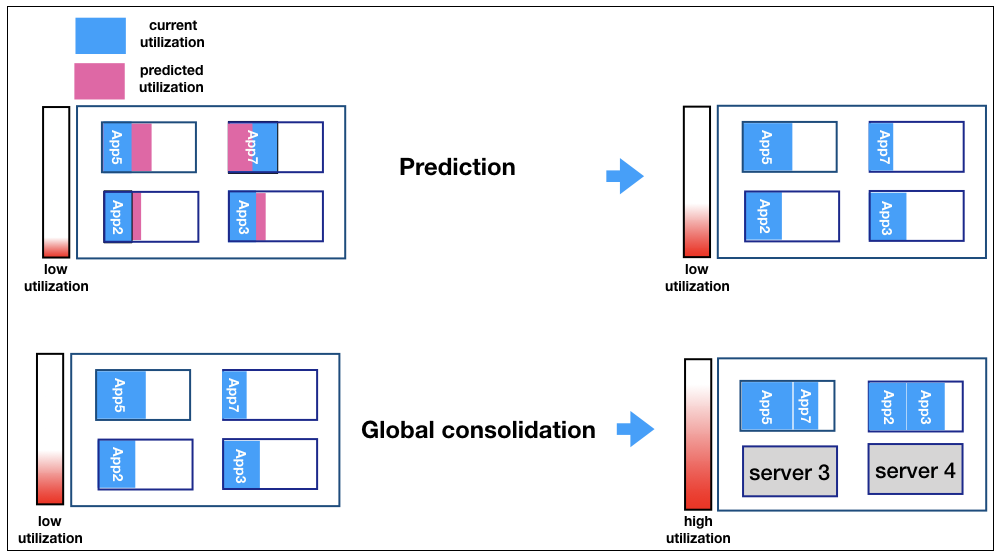
\includegraphics[width=\textwidth]{pics/predict_consolidate.png}
% 	\caption{Prediction and Consolidation}
% 	\end{subfigure}
% 	\caption{Three stages of resource management in IaaS}
% 	\label{fig:management}
% \end{figure}


% Server consolidation is the core functionality involving in all Cloud resource management operations. These operations

% Data center constantly receives new requests for applications initialization. Once the new applications have been allocated, the utilization begins to drop. This is because, initially, applications are compactly allocated on PMs. As old applications instance are released because of canceling, the compact structure become loose. Dynamic resource management is a process which can slow the utilization from decreasing. It consolidates by re-allocating one application at a time. Finally, global consolidation is conducted periodically to dramatically improve the resource utilization.
% \begin{enumerate}
% 	\item \emph{Application initialization} is applied when new applications or new VMs arrive and the problem is to allocate them into a minimum number of PMs.

% 	In this problem, a set of applications or VMs are waiting in a queue. The resource capacity of the PM and usage by applications are characterized by a vector of resource utilizations including CPU, memory and etc. Then, the allocation system must select a minimum number of PMs to accommodate them so that after the allocation, the resource utilizations remain high. The problem is to consider the different combinations of applications so that the overall resource utilization is high. This problem is naturally modeled as a static bin-packing problem \cite{CoffmanJr:1996ui} which is a NP-hard problem meaning it is unlikely to find an optimal solution of a large problem. 

% 	\item \emph{Prediction and Global consolidation} is conducted periodically to adjust the current allocation of applications so that the overall utilization is improved.

% 	In this problem, time is discrete and it can be split into basic time frames, for example: ten seconds. A periodical operation is conducted in every $N$ time frames.
% 	A cloud data center has a highly dynamic environment with continuous arriving and releasing of applications. Releasing applications cause hollow in PMs; new arrivals cannot change the structure of current allocation. Therefore, after the initial allocation, the overall energy efficiency is likely to drop along with time elapsing. 

% 	In prediction, an optimization system takes  the current applications' utilization records as the input. Make a prediction of their utilization in the next period of time. 
% 	In Global consolidation, based on the predict utilization and the current allocation - including a list of applications/VMs and a list of PMs, the system adjusts the allocation so that the global resource utilization is improved.

% 	In comparison with initialization, instead of new arrivals, the global consolidation considers the previous allocation. Another major difference is that global consolidation needs to minimize the differences of allocation before and after the optimization. This is because the adjustment of allocation relies on a technique called live migration \cite{Clark:2005uda}, and it is a very expensive operation because it occupies the resources in both the host and the target. Therefore, global optimization must be considered as a time-dependent activity which makes the optimization even difficult.

% In comparison with dynamic consolidation, global consolidation takes a set of VMs as input instead of one. Therefore, it is time consuming and often treated as a static problem.
% 	\item \emph{Dynamic resource management} 
%  	Dynamic resource management is applied in three scenarios. \textbf{First},  it is applied when a PM is overloading. In order to prevent the QoS from dropping, an application is migrated to another PM. This is called hot-spot mitigation \cite{Mishra:2012kx}. \textbf{Second}, it is applied when a PM is under-loading. Under-loading is when a PM is in a low utilization state normally defined by a threshold. At this moment, all the applications in the under-loading PM are migrated to other active PMs, so the PM becomes empty and can be turned off. This is called dynamic consolidation. \textbf{Third}, it is applied when a PM having very high level of utilization while others having low. An adjustment is to migrate one or more application from high utilized PMs to low ones. This is called load balancing.

% 	No matter which scenario it is, a dynamic resource management always involves three steps . 
% 	\begin{itemize}
% 		\item \emph{When to migrate?} refers to determine the time point that a PM is overloaded or underloaded. It is often decide by a threshold of utilization.
% 		\item \emph{Which application to migrate?} refers to determine which application need to be migrated so that it optimize the global energy consumption.
% 		\item \emph{Where to migrate?} refers to determine which host that an application is migrated to. This step is called dynamic placement which is directly related to the consolidation, therefore, it is decisive in improving energy-efficiency. 
% 	\end{itemize}

% 	Among three operations, dynamic placement is a dynamic and on-line problem.
% 	The term ``dynamic'' means the request comes at an arbitrary time point. An on-line problem is a problem which has on-line input and requires on-line output \cite{Borodin:uQcy_H6C}. It is applied when a control system does not have the complete knowledge of future events.

% 	There are two difficulties in this operation, firstly, dynamic placement requires a fast decision while the search space is very large (e.g hundreds of thousands of PMs). Secondly, migrate one application at a time is hard to reach a global optimized state.

% \end{enumerate}



% Finally, a consolidation plan includes four major items:
% 			\begin{enumerate}
% 				\item A list of existing PMs after consolidation
% 				\item A list of new virtual machines created after consolidation
% 				\item A list of old PMs to be turned off after consolidation
% 				\item The exact placement of applications and services
% 			\end{enumerate}

% By the nature of Cloud resource management, server consolidation techniques can also be categories into static and dynamic methods. Static method is a time consuming process which is often conducted off-line in a periodical fashion; initialization and global consolidation belong to this category. It provides a global optimization to the data center. Dynamic method adjusts PMs in real time. It often allocates one application at a time. Therefore, it can be executed quickly and often provides a local optimization to the data center.


















% They are bonded by the Quality of service and computing resource. Quality of service and the computing resources are the two sides of a coin. 



% Cloud users deploy their software on Clouds. They want to increase the profit by increasing income and decreasing expense. In order to accomplish this goal, they can attract more End suers by improving the functionality of softwares and the non-functionality features by guaranteeing Quality of Service (QoS). To improve the non-functionality features, Cloud users need to reserve enough resources as well as minimizing the resource so that the cost is low.

% service capacity planning is the core process. The capacity planning has two conflicting objectives, on one hand, it must meet End users' QoS requirement by using enough resources.  On the other hand, the cost must be minimized. In pre-Cloud era, the capacity planning determines the upfront investment in infrastructure, therefore, capacity, reliability, and scalability are all need to be carefully considered and balanced. In Cloud environment, the burden of capacity planning is largely released by elastic resource management and the pay-as-you-go policy.

% Cloud users identify a list of critical QoS parameters called Service Level Agreement (SLA) which specifies the non-functional requirements such as throughput, latency, and availability. These QoS parameters are mapped to resources (e.g. CPU, memory, network bandwidth) which can satisfy these requirements. Violation of SLA will lead to penalty and decreasing in number of users. Therefore, in essence, the key to attract more users is an effective resource management system which can rapidly react to the fluctuating resource demand. 

% Beside increase the income, reduce the expense is another way to improve profit. As previous section mentioned, energy consumption is the main source of expense. In energy consumption, server energy consumption is the core that needs to be improved. 

% \subsection{Energy-aware Resource Management}
% \subsection{An Overview of Evolutionary Computation}


% In order to understand Cloud computing, firstly we will illustrate the five essential elements of Cloud computing and their advantages.

% Cloud computing has five essential elements:


% \textcolor{Blue}{What is your purpose to describe the following content?}
% \textcolor{Red}{
% 	I would like to discuss the differences, advantages of disadvantage of the resource management in different service models. Therefore, after illustrate how they are work. The point is to compare the resource management. And then, lead to a new service model. And the advantage of new service model should be obvious. 
% }\\
% Traditional Cloud computing has three service model as illustrated in Figure \ref{}.
% Infrastructure as a Service (IaaS), Platform as a Service (PaaS), and Software as a Service. 
% \subsection{Resource Management}
% Scope of Cloud computing resource management.
% \begin{enumerate}
%  \item Actors
%  \item Management Objectives
%  \item Resource Types
%  \item Enabling Technologies
% \end{enumerate}






